\subsection{Current State of Tools and Research}
  \label{sec:currentState}
  There are various annotation tools designed to facilitate the generation of annotated text data sets. They are dividable into single-user and multi-user tools, i.e. for users who work alone or on only one computer and for users who want to distribute the annotation task to more than one annotator. First generations of \ac{GUI} annotation tools were single-user based like for example \textit{GATE Developer}~\cite{cunningham2011text} (started in 1995), the \textit{NITE XML Toolkit}~\cite{carletta2003nite} (2002) or \textit{WordFreak}~\cite{morton2003wordfreak} (2003) (see Figure~\ref{fig:annotationGateNiteFreak}). They all run on computers locally and are designed as individual systems, not needing a server in the background to operate. Many of them are written in Java, which makes them more platform compatible than natively complied applications. They still require to be installed on each individual computer, though.

  \begin{figure}[h]
    \centering
    \subfloat[GATE Developer]{{
      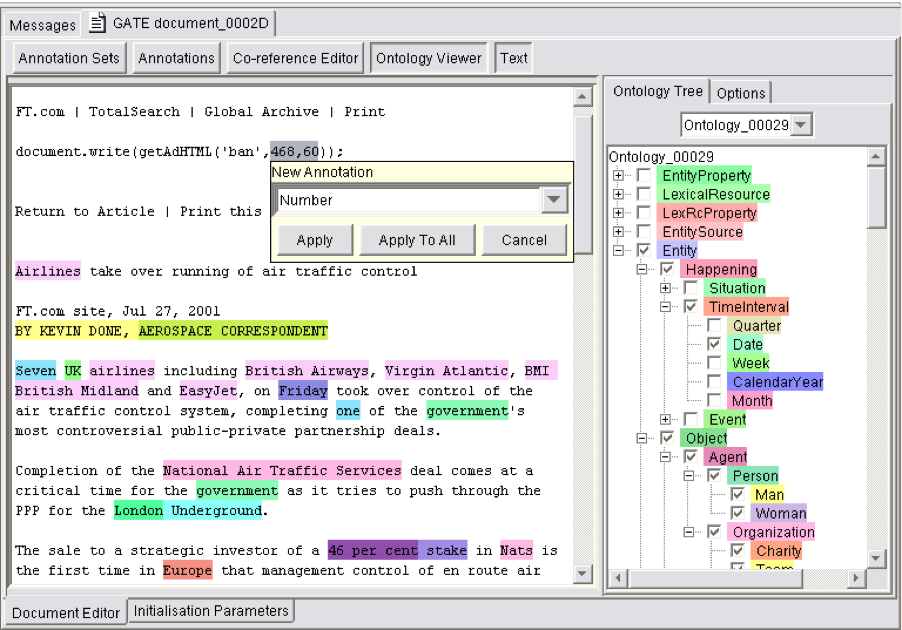
\includegraphics[width=4.1cm]{assets/1/gate.png}
    }}
    \qquad
    \subfloat[NITE XML Toolkit]{{
      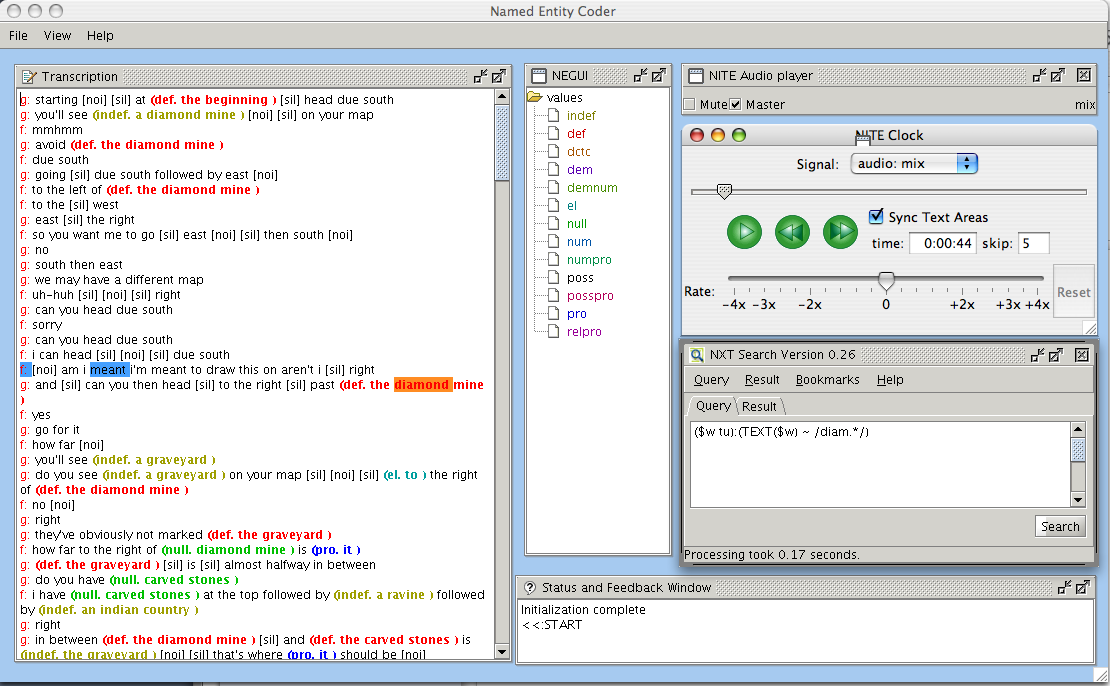
\includegraphics[width=4.1cm]{assets/1/niteXmlToolkit.png}
    }}
    \qquad
    \subfloat[WordFreak]{{
      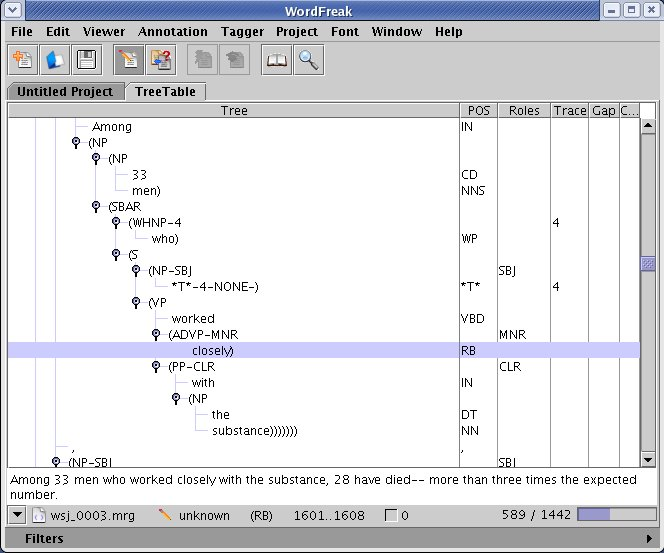
\includegraphics[width=4.1cm]{assets/1/wordFreak.jpg}
    }}
    \caption{Examples of single-user annotation tools.}%
    \label{fig:annotationGateNiteFreak}%
  \end{figure}

  In most cases modern tools belong to the multi-user class since modern web technologies have developed rapidly towards superseding native applications. Without a need for local software installation, browser based applications offer a fast access to every annotator using a browser. This reduces the requirements to participate and makes collaboration a lot easier. Collaboration is an often demanded feature to be able distribute up the workload to not only one but many annotators. Biemann et al.~\cite{biemann2017collaborative} provide a comprehensive overview of web-based, collaborative annotation tools. Not all but most of them focus on text annotation (highlighting spans and relations between spans) and thus would be in line for training data generation for the example task of this work, \ac{NER}. Two frequently used and often cited tools are \textit{GATE Teamware}~\cite{bontcheva2013gate} and \textit{WebAnno}~\cite{yimam2013webanno} (see Figure~\ref{fig:annotationGateWebanno}). Another often cited web-based annotation application is Brat~\cite{stenetorp2012brat}, which is based on Stav~\cite{ananiadou2012stav}, an annotation visualizer from the same developers.

  \begin{figure}[h]
		\centering
		\subfloat[GATE Teamware]{{
			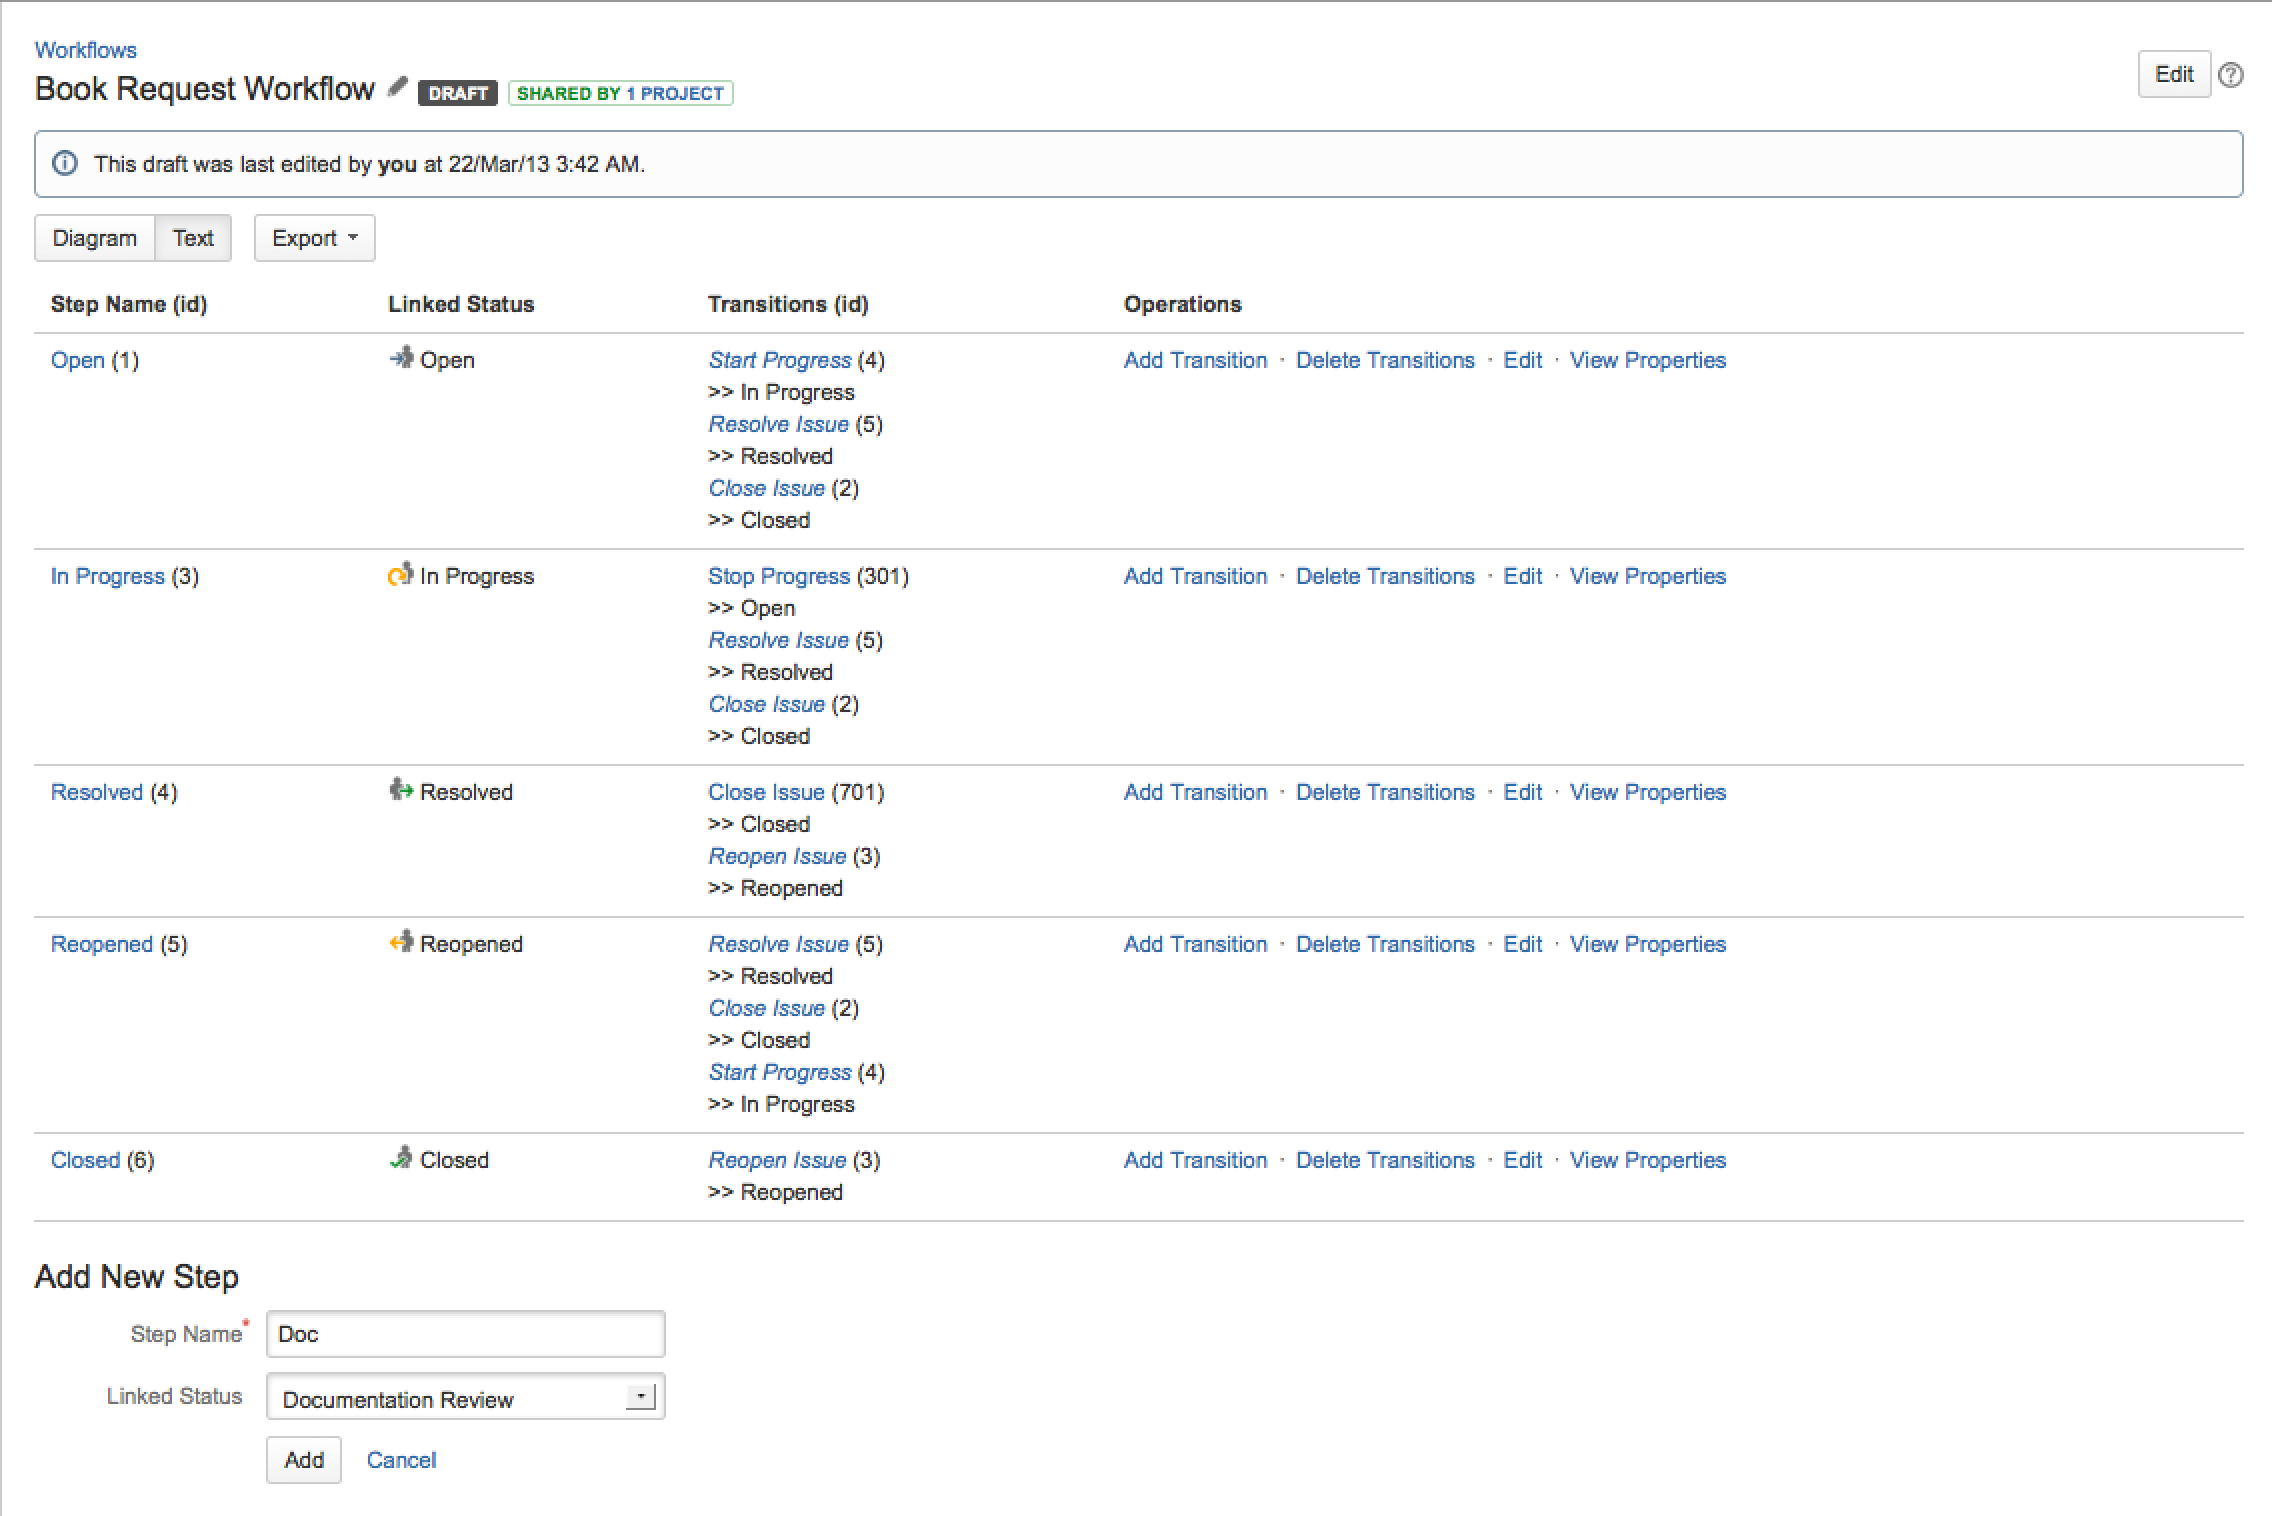
\includegraphics[width=6.7cm]{assets/1/gateTeamware.png}
		}}
		\qquad
		\subfloat[WebAnno]{{
			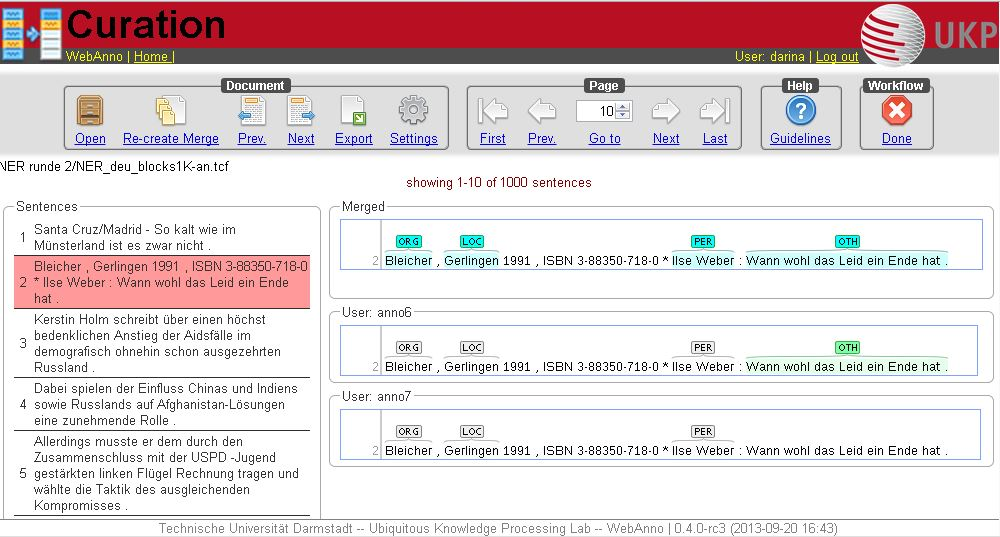
\includegraphics[width=6.7cm]{assets/1/webanno.jpg}
		}}
		\caption{Two popular web-based and collaborative text annotations tools.}%
		\label{fig:annotationGateWebanno}%
	\end{figure}

  There are various tools serving different needs like running isolated without network connectivity or as a network application with collaboration and different user roles for administration, curation and annotation. Even tools focusing on flexibility and customization with add-ons are available~\cite{biemann2017collaborative}. Some of the mentioned examples do support the the human annotator with suggestions that should help annotators doing their task: They prepare the data before the annotation and pre-label (or \lqq pre-annotate\rqq) the text to assist the human. For example GATE Teamware and WebAnno do support this feature, partly built-in and partly as a service component. It seems plausible that pre-annotations could provide a mental guidance by presenting examples for the human annotators, reduce mouse movement and thus time because not all the annotations that have to be made have to be clicked.

  Day et al.~\cite{day1997mixed}~showed as early as in 1997 that annotator productivity can be enhanced by a support system generating pre-annotations. They used a mixed-initiative setup allowing their annotators to define a rule set for pre-annotation on their own and tried to derive annotation rules from a small text set that the annotators processed before they started the annotation of the complete corpus. The derived rules were used to pre-annotate the complete corpus. The group showed an increased annotation productivity when using such pre-processed text sets, measured in processed words per minute and annotated tags per minute.

  The pre-annotation features of systems like the ones mentioned above are most of the time \ac{ML} based and try to learn from already made annotations~\cite{biemann2017collaborative}. In contrast to our approach these \ac{ML} modules use pre-trained models to predict labels. As a result, they are rather inflexible to perform on very different text domains. Moreover, they only provide pre-annotations instead of combining the output of their predictions with an \ac{AL} approach to annotate especially the sentences and paragraphs in which the model is uncertain about their annotation (see Section~\ref{sec:efficiencyAL} for further explanation). One example of an annotation tool supporting this idea is \ac{DUALIST} by Burr Settles~\cite{settles2011closing}. By using \ac{AL} and a specifically created semi-supervised learning algorithm, annotators were able to create training data sets that achieved up to \(90\%\) of the then state-of-the-art performances in only a few minutes. Settles demonstrated the usefulness of an \ac{AL} approach to create \ac{ML} models to complement the strengths of both machine and annotator~\cite{settles2011closing}.

  \paragraph{What is missing} A combination of Day's~\cite{day1997mixed} and Settle's~\cite{settles2011closing} work is desirable; a system that uses pre-annotations to assist the human doing the task and that utilizes the advantages of \ac{AL} and an iterative annotation cycle -- not only for a certain use case but for any kind of data. A validation of the impact of pre-annotations to justify developmental efforts and to be able to describe the impact on the human instead of superficial outcomes (like processed words per minute) is missing as well. As a consequence, the available work encouraged us to combine both methodologies to create a new annotation framework and to facilitate a comprehensive study: To understand the impact of pre-annotations within this new annotation environment and to go more into detail about the affected performance dimensions of human annotators.

  \pagebreak
